\chapter{Sources and the AVA catalogue}\label{sec:sources}
\section{Cross-match}
The LCO target names are not uniform (\texttt{Fairall9} and \texttt{Fairall 9}; \texttt{MCG\_08-11-011},
\texttt{MCG 8-11-11} and \texttt{MCG\_08-11-11}; \texttt{Mrk 1044} and \texttt{Mrk1044}). Each LCO name is
therefore given a position --- the median requested coordinates from the headers (\texttt{CAT-RA},
\texttt{CAT-DEC}), or the median footprint centre when no header is available --- and matched to the AVA
catalogue within 30\,arcsec (3\,arcmin for footprint positions) or by normalised name. Of the \nAva{} AVA
sources, \nAvaMatched{} are observed by the key projects (Fig.~\ref{fig:sky}); \avaMissing{} are not. \nAvaReview{}
matches by name have discrepant positions and are flagged for inspection.

The AVA table is the master target list. Every frame in both databases carries the AVA identifier of its target
(\texttt{frames.ava\_id} and \texttt{ava\_data\_id}; the name-to-identifier links are in table
\texttt{target\_link}), refreshed at every daily update, so any image or spectrum can be selected by AGN regardless
of how its target was named at the telescope. Manual decisions (for example, the offset fields of NGC~4395) go in
\texttt{AVA/ava\_link\_overrides.csv} and take precedence over the automatic match. The AVA table itself is also
kept as an SQLite database, \texttt{AVA/ava.sqlite} (the original table verbatim in \texttt{agn}, the recomputed LCO
statistics in \texttt{agn\_lco}, and the links in \texttt{lco\_targets}), with two CSV copies: \texttt{ava.csv}
(all columns, with header) and \texttt{ava\_nohead.csv} (the original columns, without header, byte-identical to
the master rows).

The LCO columns of the AVA table are refreshed from the databases (Table~\ref{tab:ava}) in a new file
\texttt{AVA/ava\_lco\_updated.csv}, which keeps the previous values (\texttt{*\_prev}) and leaves the Swift and
Liverpool Telescope columns untouched. The counts include only the key projects listed in
Table~\ref{tab:proposals}; the earlier AVA values for some sources also included other programmes (e.g.\ AGN
STORM~2 for Mrk~817), so a lower number is not a loss of data. Cadences are medians of the intervals between visits.

\begin{figure}[h]
\centering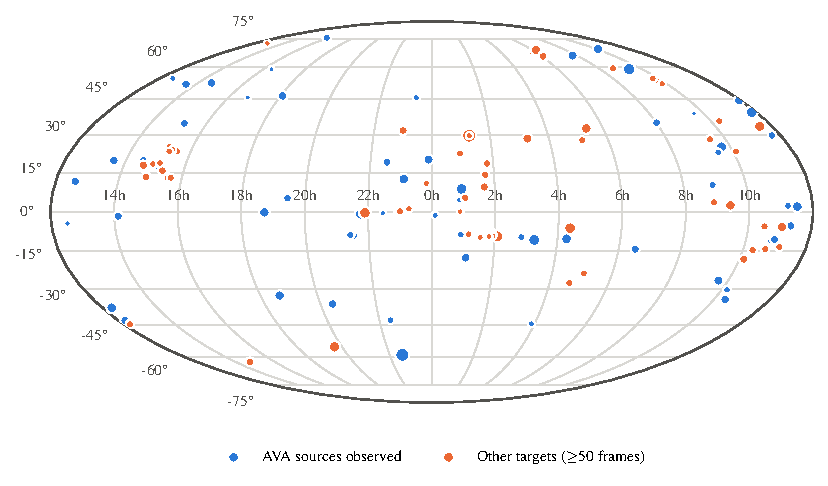
\includegraphics[width=0.9\textwidth]{figures/fig_sky.pdf}
\caption{Sky positions of the AVA sources observed by the key projects and of other LCO targets with at least
50 frames; symbol size grows with the number of frames.}\label{fig:sky}
\end{figure}

\begin{small}
\setlength{\tabcolsep}{4pt}
\begin{longtable}{lrrrlrrlp{2.4cm}}
\caption{LCO holdings of the AVA sources: reduced images, visits, median imaging cadence (d), imaging dates,
FLOYDS epochs, median spectroscopic cadence (d), FLOYDS dates and the key projects that observed it
(e.g.\ 23Bf = KEY2023B-001f).}\label{tab:ava}\\
\toprule
Source & Images & Visits & Cad. & Imaging & Ep. & Cad. & FLOYDS & KP \\
\midrule\endfirsthead
\toprule
Source & Images & Visits & Cad. & Imaging & Ep. & Cad. & FLOYDS & KP \\
\midrule\endhead
\inputtable{tables/tab_ava.tex}
\bottomrule
\end{longtable}
\end{small}

\section{Properties of the sample}
Table~\ref{tab:properties} lists the AVA sources with their redshift, Galactic reddening, mean $g$ magnitude,
luminosity, Eddington ratio and black-hole mass from the AVA catalogue, and the imaging and FLOYDS cadences
measured from the database.

\begin{small}
\setlength{\tabcolsep}{3.5pt}
\begin{longtable}{lccccccccrr}
\caption{The AVA sample, ordered by right ascension. $z$, E($B-V$), $g$ (mean LCO magnitude), $\log L$,
$L/L_{\rm Edd}$ and $\log M_{\rm BH}$ are from the AVA catalogue; the cadences are the median intervals between
LCO imaging visits and between FLOYDS epochs in the key projects (Table~\ref{tab:proposals}).}\label{tab:properties}\\
\toprule
Name & RA & Dec & $z$ & E($B-V$) & $g$ & $\log L$ & $L/L_{\rm Edd}$ & $\log M_{\rm BH}$ & LCO cadence & FLOYDS cadence \\
 & hh mm ss.s & $\pm$dd mm ss & & & mag & erg\,s$^{-1}$ & & M$_\odot$ & day & day \\
\midrule\endfirsthead
\multicolumn{11}{l}{\small\itshape Table \ref{tab:properties} -- continued}\\
\toprule
Name & RA & Dec & $z$ & E($B-V$) & $g$ & $\log L$ & $L/L_{\rm Edd}$ & $\log M_{\rm BH}$ & LCO cadence & FLOYDS cadence \\
 & hh mm ss.s & $\pm$dd mm ss & & & mag & erg\,s$^{-1}$ & & M$_\odot$ & day & day \\
\midrule\endhead
\bottomrule\endfoot
\inputtable{tables/tab_properties.tex}
\end{longtable}
\end{small}

\section{Targets not in the catalogue}
\nNotInAva{} LCO target names have no AVA counterpart; \nNotInAvaFifty{} of them have at least 50 frames.
They include AGN that should be added (Table~\ref{tab:new}) as well as photometric comparison fields and
short test observations.

\begin{small}
\begin{longtable}{lrrrr}
\caption{LCO targets without an AVA counterpart, by number of frames (first 40).}\label{tab:new}\\
\toprule
LCO name & RA (deg) & Dec (deg) & Images & Spectra \\
\midrule\endfirsthead
\toprule
LCO name & RA (deg) & Dec (deg) & Images & Spectra \\
\midrule\endhead
\inputtable{tables/tab_new.tex}
\bottomrule
\end{longtable}
\end{small}
